
\documentclass[runningheads]{llncs}
\usepackage{graphicx}
\usepackage{bibentry}
\usepackage{amsmath}
\usepackage{nccmath}
\usepackage{float}
\usepackage{multirow}
\usepackage{algorithm}
\usepackage{xfrac}
\usepackage[noend]{algpseudocode}
\nobibliography*

\begin{document}
%
\title{Mitigation of Bias in Data to Achieve Fairness-Aware Classification}

\author{Pooja Hanavadi Balaraju\inst{1}} 
%
%\authorrunning{F. Author et al.}

\institute{RWTH Aachen University
\email{pooja.balaraju@rwth-aachen.de}\\
}
%
\maketitle              % typeset the header of the contribution
%--------------------------------------------------------------------------------
\begin{abstract}
Machine learning has seen a rapid growth in recent years in a variety of sectors and services. Automated decision making uses machine learning techniques to remove human interference . It predicts the decision based on past experience of similar situation but makes it challenging because the predictions need to match with accuracy. However, one its major concerns is misclassification errors caused due to bias in the training data. These errors put certain sensitive groups at an unfair advantage creating different types of unfairness: disparate impact, disparate treatment and disparate mistreatment. Therefore fairness concerns have become increasingly important. In this paper, we discuss some of the current methodologies developed recently to mitigate bias and achieve fairness like massaging of the labels, group thresholding, covariance and adaptive sensitive reweighting. We learn that it is unsufficient to remove the sensitive information for eliminating biases because it has an indirect correlation. We analyse and compare the performance of these methods based on different fairness metrics for three  datasets. We observe that adaptive sensitive reweighting model achieves better or similar trade-offs between accuracy and unfairness mitigation when compared to other fairness-aware approaches.
 

\keywords{Machine Learning  \and Classifier \and Unfairness}
\end{abstract}
%-------------------------------------------------------------------------------
\section{Introduction}
Machine learning is a brach of artificial intelligence in which systems can learn from data or experience to make decisions with minimal human intervention. It is growing across many fields because it can analyze large amount of data to identify patterns in a short interval of time. Some of the major appplications are: speech recognition, email spam and malware filtering, search engine result refininng and automated decisition making process and so on.\\
With the increase in shift towards automated decision making process of machine learning in various services that affects people's lives, there is an immense need for fairness concerns. The decisions should be unbiased and nondiscriminatory in relation to the sensitive features such as gender, sex, religion, race and so on. These sensitive features should be carefully treated, and if not constrained well, it leads to bias in the decision making process which gives an unfair treatment to certain people based on sensitive attributes. For example, training a logistic regression classifier on the ProPublica COMPAS dataset of crime recidivism \cite{compasdataset} yields differences between black and white defendants that amount to 17\% for false positives and 25\% for false negative rates \cite{krasanakis2018adaptive}.\\
Researchers have previously recognized that classification is often caused by data rather than classifier \cite{feldman2015certifying} \cite{kleinberg2016inherent}. Elimination of sensitive features from data is insufficient for avoiding misclassification, due to the indirect influencec of the sensitive information. For example, when determining credit scoring, let us remove the sensitive feature race. People of a specific race live in a specific area and address is used as a feature for training the prediction model, then we can expect unfair determinations even though race is not considered. This is called a red-lining effect \cite{calders2010three} or indirect discrimination \cite{pedreshi2008discrimination}. This happens due to inherent inability to treat datasets and we discuss some of the reasons in the section 5.\\
In this paper, we discuss the following methods to mitigate bias in the training data:
\begin{itemize}
\item Group Thresholding: The goal of this method is to predict a true outcome $Y$ from features $X$ based on labeled training data, while ensuring the prediction is "non-discriminatory" with respect to a specified protected attribute $A$ \cite{hardt2016equality}.
\item Regularizer: Adjusting regularizers to reduce indirect prejudice (statistical dependence between sensitive information) to restrict learner's beahviour \cite{kamishima2012fairness}.
\item Covariance : Convex concave programming is used to reduce the different unfairness measures discussed in the next section \cite{zafar2017fairness} \cite{zafar2015fairness}.
\item Adaptive-Sensitive Reweighting : Assumes that there exists an underlying set of class labels corresponding to training samples, that if, predicted would yield unbiased classfification with respect to a fairness objective. Weights are obtained using the CULEP model that stands for Convex Underlying Label Error Pertubation \cite{krasanakis2018adaptive}.
\end{itemize} 
The structure of the paper is as follows: Section 2 discusses the background and related work. Section 3 constitutes the different methodolgies explained in detail. Section 4 provides information about dataset editing deficiencies. Section 5 provides information on the experiments conducted along with the results depicting the performance analysis of each of the methods. Section 6 concludes the paper summarizing the results and the future work.
%-------------------------------------------------------------------------------
\section{Background and Related Work}
In this section we first elaborate on the different types of unfairness  and their corresponding metrics used to measure them in automated decision making process. Throughout this paper, we consider binary classifiers that produce label estimations $\tilde{y_i} \in \{0,1\}$ for samples $i$ of features $x_i$ and labels $y_i \in \{0,1\}$. If a certain group of sample is associated with the sensitive attributes then they are considered as sensitive samples $S$ and the non-sensitive complement $S'$.
\subsection{Types of Unfairness}
Classification unfairness is often expressed through the notions of disparate treatment, disparate impact and disparate mistreatment \cite{zafar2015fairness}. Let us take an example of \cite{zafar2017fairness} to illustrate the three types of unfairness. The classifier needs to decide whether or not to stop a person on suspicion of having an illegal weapon based on set of features like bulge in clothing and proximity to a crime scene. The ground truth tells whether a person actually possesses an illegal weapon or not. 
\begin{table}[!htbp]
    \begin{minipage}{.40\linewidth}
      \centering
\begin{tabular}{c|c|c}
\hline
\multicolumn{3}{c}{User Attributes}\\
\hline
Sensitive & \multicolumn{2}{c}{Non-Sensitive} \\
\hline
Gender   & Clothing Bulge    & Prox Crime\\
\hline
Male1   &  1 & 0\\
\hline
Male2   &  1 & 0\\
\hline
Male3   &  0 & 1\\
\hline
Female1   &  1 & 1\\
\hline
Female2   &  1 & 0\\
\hline
Female3   &  0 & 0\\
\hline
\end{tabular}
\end{minipage}%
    \begin{minipage}{.40\linewidth}
      \centering
        \begin{tabular}{c}
        \hline
Ground Truth \\
(Has Weapon) \\
\\
\hline
y\\
\hline
y\\
\hline
n\\
\hline
y\\
\hline
n\\
\hline
y\\
\hline
\end{tabular}
\end{minipage}%
    \begin{minipage}{.20\linewidth}
      \centering
        \begin{tabular}{c|c|c}
        \hline
\multicolumn{3}{c}{Classifier's} \\
\multicolumn{3}{c}{Decision to Stop} \\
\hline
$C_1$   &	$C_2$    &	$C_3$\\
\hline
1   &  1 & 1\\
\hline
1   &  1 & 0\\
\hline
1   &  0 & 1\\
\hline
1   &  0 & 1\\
\hline
1   &  1 & 1\\
\hline
0   &  1 & 0\\
\hline
\end{tabular}
\end{minipage}%
\\
\caption{Decision of three classifiers ($C_1$, $C_2$ and $C_3$) on whether (1) or not (0) to stop a pedestrian on the suspicion of possessing an illegal weapon}
\label{fig:disparates}
\end{table}
\begin{enumerate}
\item Disparate treatment elimination: ability of a trained classifier to yield the same output $\hat{y_i}$ for features $x_i$ irrespective of the sample belonging to the sensitive group $S$ or the non-sensitive group $S'$ \cite{krasanakis2018adaptive}.
\begin{equation}
P(\hat{y_i}|x_i, i \in S) = P(\hat{y_i}|x_i)
\label{eq:disparatetreatment}
\end{equation}
As seen in \ref{fig:disparates}, $C_2$ and $C_3$ are unfair due to disparate treatment since $C_2'$s and $C_3'$s decisions for Male1 and Female1 are different even though they have the same values of non-sensitive attributes \cite{zafar2017fairness}.
\item Disparate impact elimination: ability of a classifier to achieve statistical parity |cite{kamiran2012data} \cite{kamiran2010discrimination} \cite{kamishima2012fairness} i.e, assigns the same portion of the users to a class for sensitive and non/sensitive groups \cite{krasanakis2018adaptive}.
\begin{equation}
P(\hat{y_i} = 1|i \in S) = P(\hat{y_i} = 1|i \notin S)
\label{eq:disparateimpact}
\end{equation}
As depicted in Fig. \ref{fig:disparates}, $C_1$ is unfair due to disparate impact because the fraction of males and females that were stopped are different (1.0 and 0.66 respectively) \cite{zafar2017fairness}.
\item Disparate mistreatment elimination: ability of a classifier to achieve equal misclassification rates across sound ground truth tables(i.e. not suffering from dataset construction problems, such as historical biases) \cite{zafar2015fairness} \cite{zafar2017fairness} \cite{krasanakis2018adaptive}. For example, if the race is a sensitive attribute for prediction of criminal behaviour \cite{compasdataset}, disparate mistreatment elimination would ensure the same error rate between white and non-white defendants \cite{krasanakis2018adaptive}. The most common mistreatment constraint is equal number of false positive rates(FPR) and false negative rates (FNR).
\begin{equation}
\begin{split}
P(\hat{y_i} \neq y_i | y_i = 1,i \in S) = P(\hat{y_i} = 1|i \neq y_i | y_i = 1,i \notin S) \\
P(\hat{y_i} \neq y_i | y_i = 0,i \in S) = P(\hat{y_i} = 1|i \neq y_i | y_i = 0,i \notin S)
\label{eq:disparatemis}
\end{split}
\end{equation}
Fig. \ref{fig:disparates} shows that $C_1$ and $C_2$ are unfair due to disparate mistreatment because their rate of erroneous decisions for males and females are different: $C_1$ has different false negatives for males and females (0.0 and 0.5 respectively) \cite{zafar2017fairness}.
\end{enumerate}
%--------------------------------------------------------------------------------
\subsection{Metrics}
Disparate treatment and disparate impact is measured using $p\%$ rule. The $p\%$ \cite{biddle2006adverse} rule is an empirical rule which does not allow sensitive group identification to be lower than a set percentage of non-sensitive group identification:
\begin{equation}
pRule = min\{\frac{P(\hat{y_1}|i \in S)}{P(\hat{y_1}|i \notin S)},\frac{P(\hat{y_1}|i \notin S)}{P(\hat{y_1}|i \in S)}\}
\label{eq:prule}
\end{equation}
Let us consider a specific instantiation supported by the U.S Equal Employment Opportunity Commission: the  "80\%-rule". The $p\%$ rule states that the ratio between the percentage of subjects having a certain sensitive attribute value assigned the positive decision outcome and the percentage of subjects not having the value also assigned the positive outcome should be non less than p:100 \cite{zafar2015fairness}.\\
On the other hand, the disparate mistreatment elimination conditions in Eq. \ref{eq:disparatemis}, it is measured using the following measures \cite{krasanakis2018adaptive}:
\begin{equation}
\begin{split}
D_{FPR} = P(\hat{y_i} | y_i = 1, i \in S) - P(\hat{y_i} | y_i = 1, i \notin S) \\
D_{FNR} = P(\hat{y_i} | y_i = 0, i \in S) - P(\hat{y_i} | y_i = 0, i \notin S)
\label{eq:disparatefprfnr1}
\end{split}
\end{equation}
The overall disparate mistreatment is a combination of the above two metrics:
\begin{equation}
|D_{FPR}| + |D_{FNR}|
\label{eq:disparatefprfnr2}
\end{equation}
%--------------------------------------------------------------------------------
\subsection{Related Work}
Methodologies to reduce bias can be boradly classified into the following groups:
\begin{enumerate}
\item Preprocessing the training data: this is based on the assumption that disparate impact of the trained classifier is due to the disparate impact on the training data. In order to avoid the disparate impact, the sensitive attributes are ignored. However, ignoring the sensitive attribute information may still lead to disparate impact in outcomes: since automated decision making systems are often trained on historical data , if a group with certain sensitive attribute was unfairly treated in the past, this unfairness may persist in future predictions through indirect discrimination, leading to disparate impact \cite{zafar2015fairness}. These approaches include massaging the dataset \cite{calders2009building} \cite{kamiran2009classifying} \cite{kamiran2012data} \cite{vzliobaite2011handling} by changing class labels that are identified as mislabeled due to bias and reweighting training samples so that more importance is places on sensitive sttributes \cite{calders2009building} \cite{kamiran2012data}.
\item Training under fairness constraints: solves disparate impact by adjusting the training rules by editing the rules themselves \cite{calders2013controlling} \cite{zafar2015fairness} or by introducing linear programs constraints \cite{celis2017ranking} \cite{dwork2012fairness} \cite{romei2014multidisciplinary} \cite{zafar2015fairness}.
\item Edit posteriors: these methods attempt to edit posteriors to satisfy fairness coonstrains but requires information about the sensitive group to make appropriate decisions \cite{dionne2014economic} \cite{doherty2012information} \cite{feldman2015computational} \cite{hardt2016equality}. 
\end{enumerate}
%---------------------------------------------------------------------------------
\section{Methodology}
In this section, we will discuss some of the methods that have been proposed to mitigate bias in the traning data to achieve accuracy.
\subsection{Adaptive Sensitive Reweighting + CULEP}
Analysis is conducted on binary probabilistic classifier, which produces probability estimates $\hat{P}(Y=y_i) = 1 - \hat{P}(Y \ne y_i)$ for samples $i$ with features $x_i$ and each class label $Y \in \{0,1\}$. This classifier estimates class labels as:
\begin{equation}
\hat{y_i} = argmax\hat{P}(Y=y_i) = argmin\hat{P}(Y \ne y_i) , Y \in \{0,1\}
\end{equation}
A well-calibrated classifier has the misclassification error $P(Y \ne y_i)$ reaching a minimization target in the learning process. For the training sample $i$, features $x_i$ and class labels $y_i$, there exists underlying class labels $\tilde{y_i}$ (unobservable) that yields estimated labels $\hat{y_i}$ which conforms to designated fairness and accuracy trade-offs. Training goals are two-fold: a) make the calssifier yield accurate predictions, minimize $\hat{P}(\hat{y_i} \ne y_i)$ and b) make classifier predictions approach the underlying labels, minimize ${\hat{P}(\hat{y_i} \ne y_i)}^2$. It is difficult to attain both of them when the original labels do not coincide with the underlying labels. 
\begin{figure}[H]
\begin{minipage}{.5\textwidth}
  \centering
  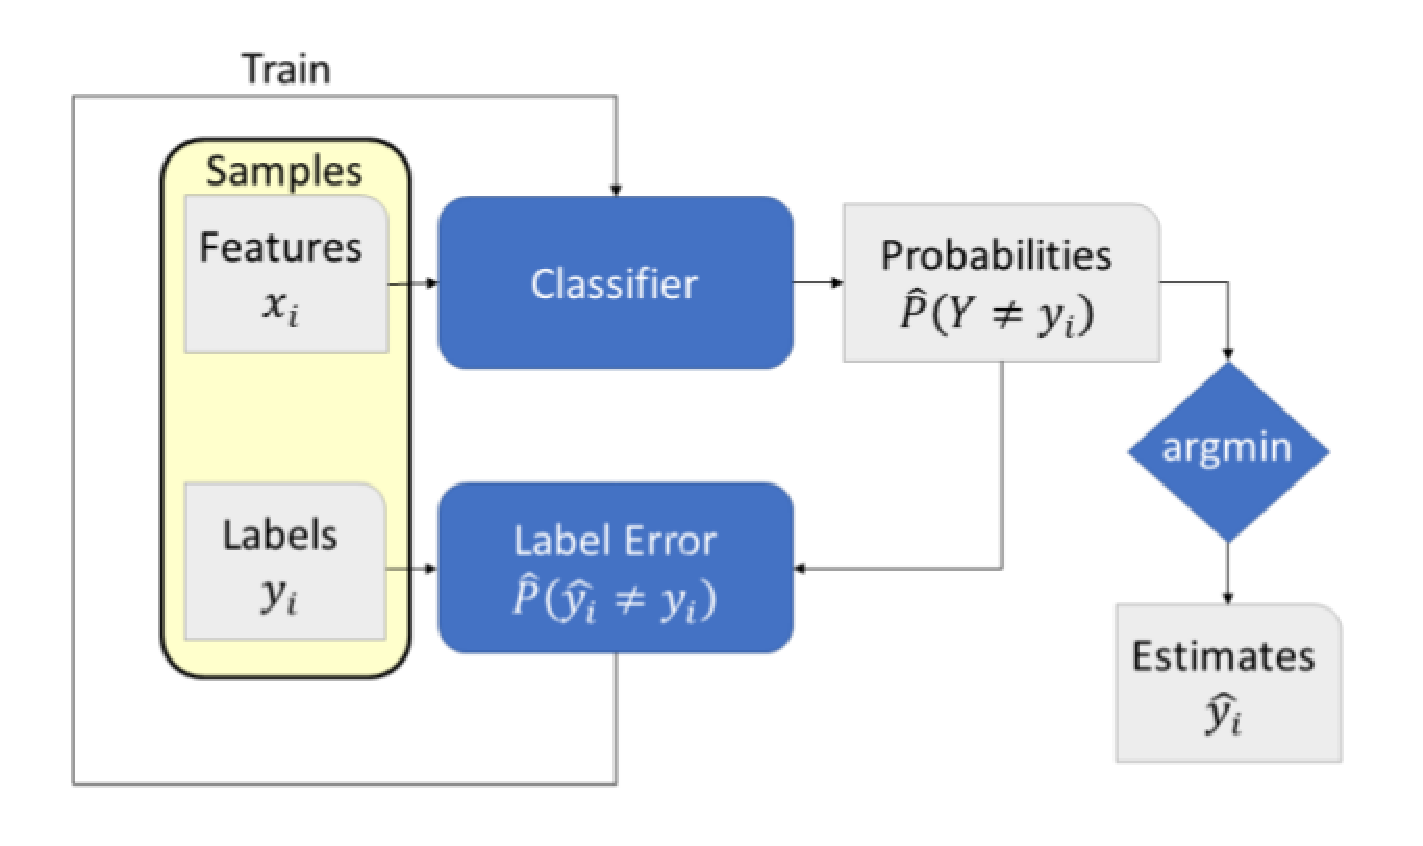
\includegraphics[width=\linewidth]{img/Fig1.eps}
  \caption{Probabilistic classifier training}
  \label{fig:datalabels}
\end{minipage}%
\begin{minipage}{.35\textwidth}
  \centering
  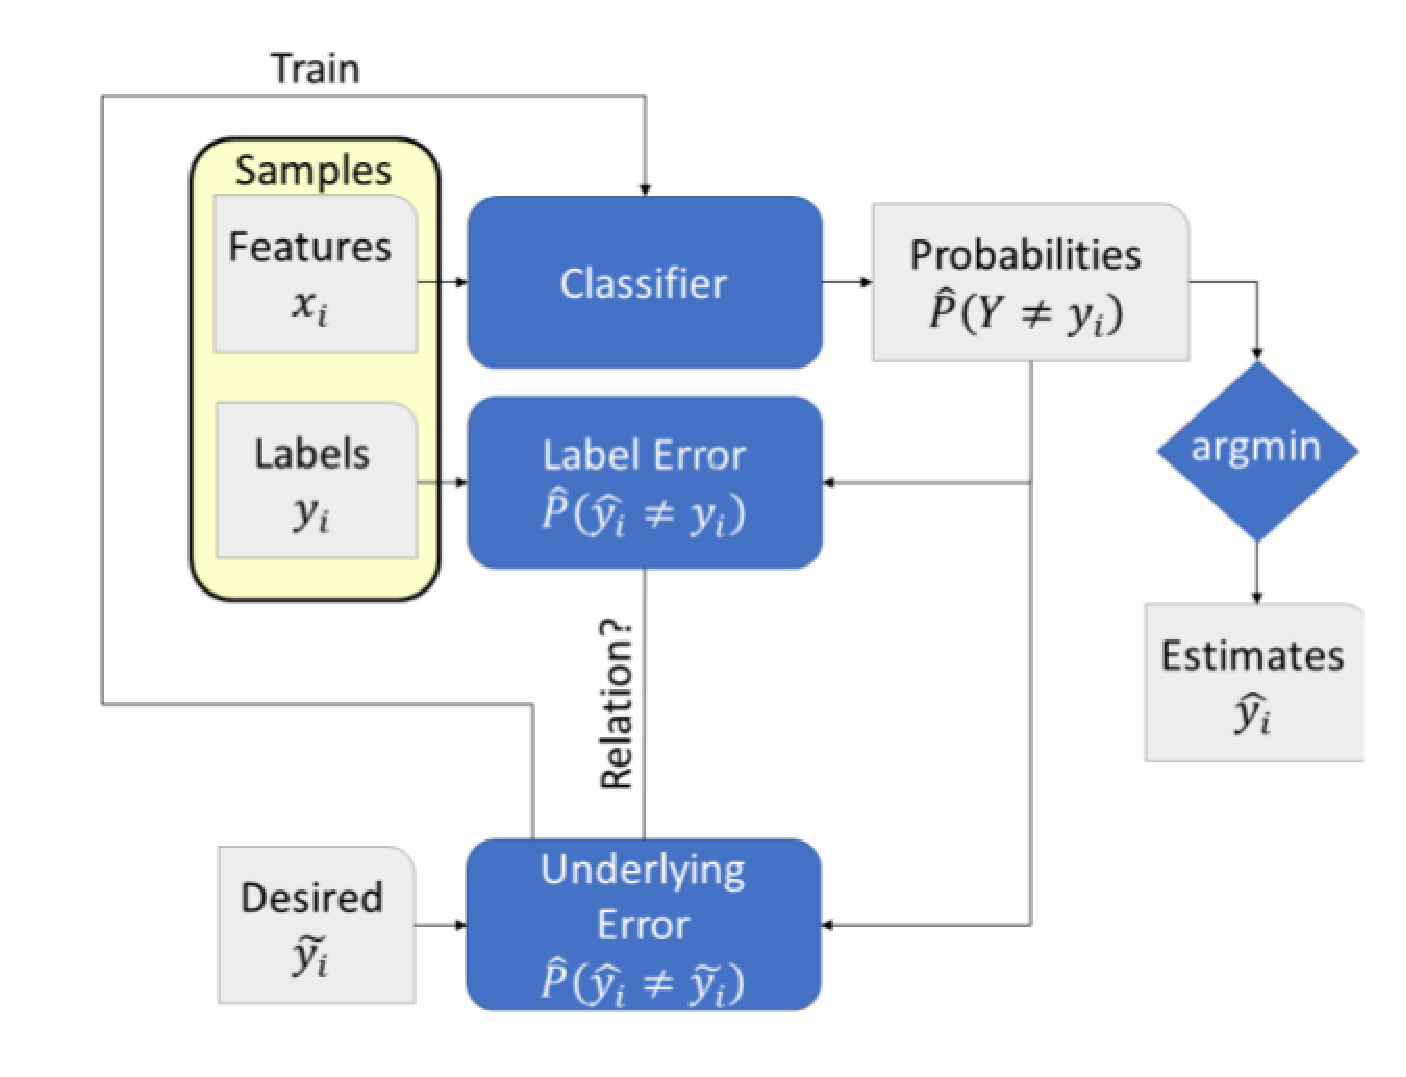
\includegraphics[width=\linewidth]{img/Fig2.eps}
  \caption{Directly training on observable desired labels}
  \label{fig:underlabels}
\end{minipage}
\end{figure}
Training the data labels could be achieved using the mechanism in Fig \ref{fig:datalabels}and training towards underlying labels could be done using the mechanism in Fig \ref{fig:underlabels}.However, estimating the underlying labels and directly using them for training is considered under data falsification under legal constraints. In order to solve this contradiction, weights $w_i$ are trained on the data labels which makes them equivalent to the unweighted training on the underlying labels. The goal is now is to minimize the weighted error and also bridge the gap between the weighted data labels and unweighted underlying labels.
\begin{equation}
min\sum_{i=1}{w_i\hat{P}(\hat{y_i} \ne y_i)} \\
\label{eq:objective1}
\end{equation}
\begin{equation}
min\sum_{i=1}{\{w_i\hat{P}(\hat{y_i} \ne y_i) - \hat{P}(\hat{y_i} \ne \tilde{y_i})}\}^2 
\label{eq:objective2}
\end{equation}
We equate Eq.\ref{eq:objective2} to 0 which yields us:
\begin{equation}
w_i\hat{P}(\hat{y_i} \ne y_i) = \hat{P}(\hat{y_i} \ne \tilde{y_i})
\label{eq:objective2}
\end{equation}
\begin{figure}[H]
  \centering
  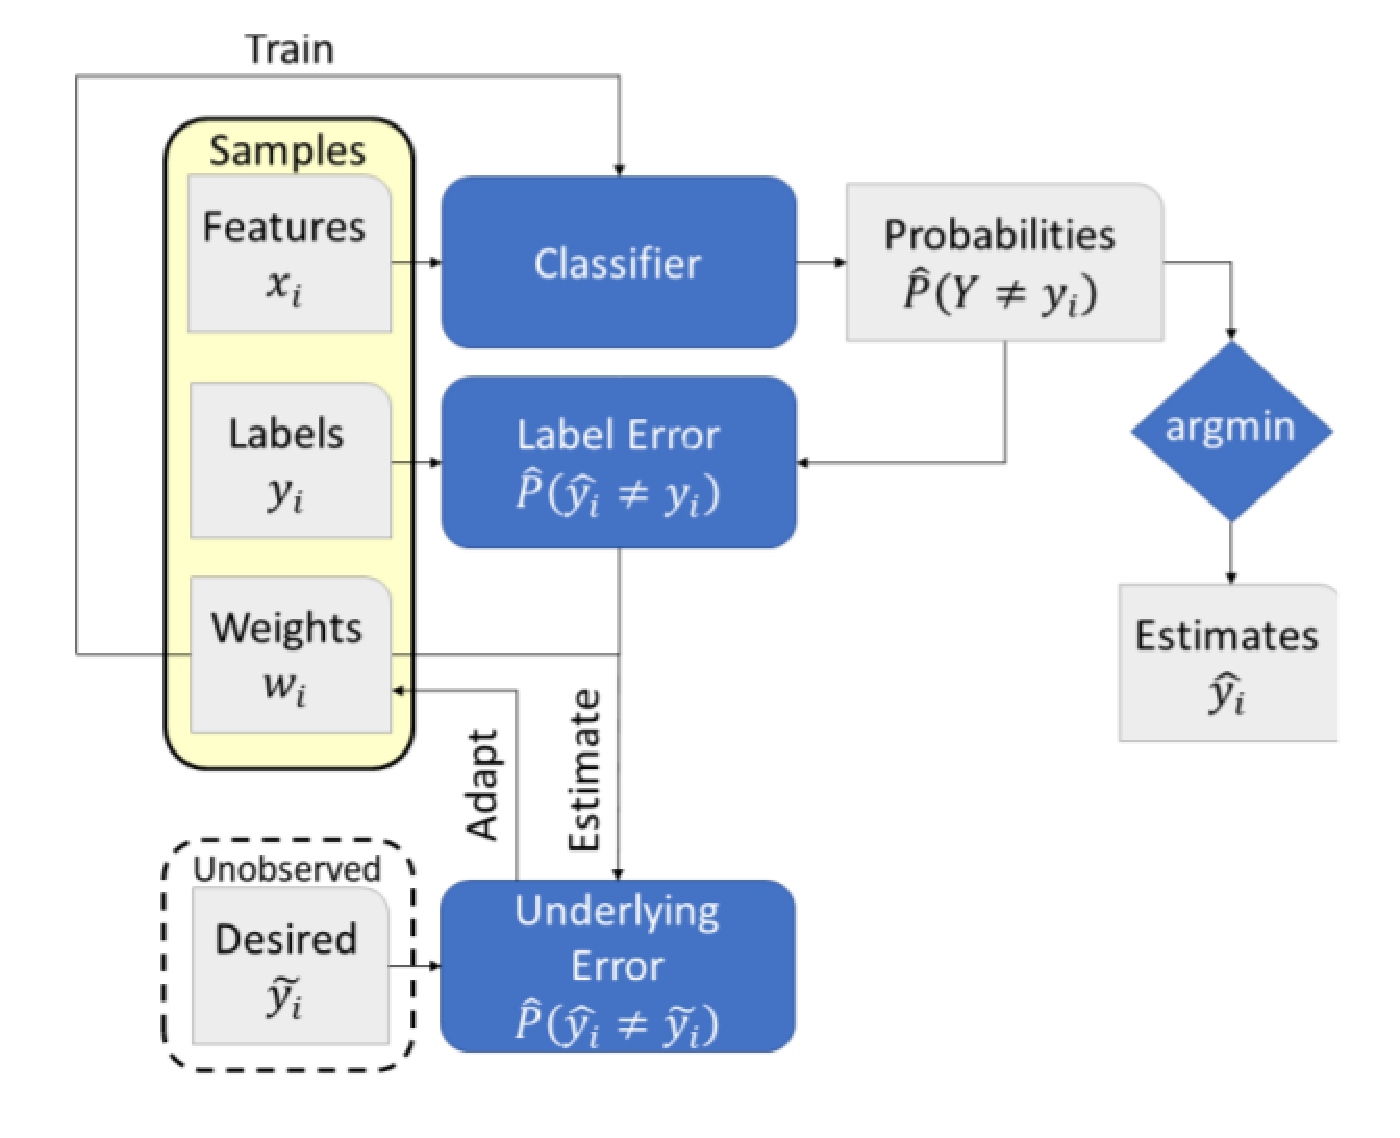
\includegraphics[width=0.5\linewidth]{img/Fig3.eps}
  \caption{Training on unobservable desired labels}
  \label{fig:unobservelabels}
\end{figure}
The authors in \cite{krasanakis2018adaptive} have proposed a model which employs conditional probabilities to make informed estimations based on $\hat{P}(\hat{y_i} \ne y_i)$. This model achieves the goals by estimating the underlying labels while training on weighted original labels as seen in Fig.\ref{fig:unobservelabels} .This process shifts the focus from the training scheme to discovering probability estimation model that can train towards the goal than searching explicitly searching for underlying labels. The advantages of using this model are three fold: a) the classifier is not accuse of being trained on falsified data, b) selection of estimation models that trains towards objectives that could not be formulated as deficiencies in training data and c)there is no need to introduce massaging heuristics to distribute the relabeling.\\
\begin{algorithm}
\caption{Adaptive Sensitive Reweighting}\label{euclid}
\begin{algorithmic}[1]
\Function{REWEIGHT}{Classifier $C$, Data $D$, Sensitive Group $S$}
\State $w_i \leftarrow \forall i \in D$
\State $w_i,prev \leftarrow 1 + \sqrt{e} \forall i \in D$
%\BState \emph{top}:
\While {$\sum_{i \in D}\{w_i-w_i,prev\}^2 \geq e$} 
\State Train $C$ samples: $i = (x_i,y_i) \in D$ and weights $\frac{w_j}{\sum_{j \in D}{w_j}}$.
\State Use $C$ to Obtain $\hat{P}(\hat{y_i} \notin y_i)$.
\State Estimate $\hat{P}(\hat{y_i} \notin \tilde{y_i})$ using $\hat{P}(\hat{y_i} \notin y_i) \forall i \in D$.
\State $w_i,prev \leftarrow w_i \forall i \in D$
\State $w_i \leftarrow \sfrac{P(\hat{y_i} \neq \tilde{y_i})}{P(\hat{y_i} \neq y_i)} \forall \in D$
\EndWhile
\Return trained classifier $C, \{w_i\}$
\EndFunction
\end{algorithmic}
\end{algorithm}

The weights are determined using the Convex Underlying Label Error Pertubation (CULEP) model. When the original labels coincide with the underlying labels we expect overfitting and similarly when they do not coincide, we expect underfitting. This is represented as follows:
\begin{equation}
(\hat{P}(\hat{y_i} \neq \tilde{y_i} | y_i = \tilde{y_i})-\hat{P}(\hat{y_i} \neq y_i))(\hat{P}(\hat{y_i} \neq \tilde{y_i} | y_i \neq \tilde{y_i})-\hat{P}(\hat{y_i} \neq y_i)) < 0
\label{eq:overunderfit}
\end{equation}
To satisfy this property the authors in \cite{krasanakis2018adaptive} propose conditional probabilities by pertubating classifier error of training samples $i$. To achieve this, they multiply it with values of a non-decreasing convex function $L_{\beta i}(p_i) \geq 0$, $L_{\beta i}(0) = 1$ of pertubation paramters $p \in [-1,1]$ whose Lipschitz constant is proportional to $\beta_i^3$. Depending on overestimatio(+) or underestimation Eq. \ref{eq:overunderfit} can be represented as:
\begin{equation}
\begin{split}
\hat{P}(\hat{y_i} \neq \tilde{y_i} | y_i = \tilde{y_i}) = L_{\beta i}(\pm \hat{P}(\hat{y_i} \neq y_i))\hat{P}(\hat{y_i} \neq y_i) \\
\hat{P}(\hat{y_i} \neq \tilde{y_i} | y_i = \tilde{y_i}) = L_{\beta i}(\mp \hat{P}(\hat{y_i} \neq y_i))\hat{P}(\hat{y_i} \neq y_i) 
\end{split}
\label{eq:lipschitz}
\end{equation}
The authors have selected different Lipschitz constants for the senstive group $S$ and the non-sensitive group $S'$ as follows:
\begin{equation}
\begin{split}
\beta_i = \beta_s | i \in S\\
\beta_i = \beta_{s'} | i \notin S\\
\end{split}
\label{eq:lipschitzconstants}
\end{equation}
Conditional probability needs to consider the probability bias for inadequate labeling. Data mislabeling would occur with a fixed probability, depending on whether samples belong to the sensitive group which can be modeled as two Bernoulli processes, one for the sensitive group $S$ and the other for the non-sensitive group $S'$ as follows:
\begin{equation}
\begin{split}
\beta_i = \beta_s | i \in S\\
\beta_i = \beta_{s'} | i \notin S\\
\end{split}
\label{eq:lipschitzconstants}
\end{equation}
%---------------------------------------------------------------------------------
\subsection{A Subsection Sample}
Please note that the first paragraph of a section or subsection is
not indented. The first paragraph that follows a table, figure,
equation etc. does not need an indent, either \cite{test1}.

Subsequent paragraphs, however, are indented.

\subsubsection{Sample Heading (Third Level)} Only two levels of
headings should be numbered. Lower level headings remain unnumbered;
they are formatted as run-in headings.

\paragraph{Sample Heading (Fourth Level)}
The contribution should contain no more than four levels of
headings. Table~\ref{tab1} gives a summary of all heading levels.

\begin{table}
\caption{Table captions should be placed above the
tables.}\label{tab1}
\begin{tabular}{|l|l|l|}
\hline
Heading level &  Example & Font size and style\\
\hline
Title (centered) &  {\Large\bfseries Lecture Notes} & 14 point, bold\\
1st-level heading &  {\large\bfseries 1 Introduction} & 12 point, bold\\
2nd-level heading & {\bfseries 2.1 Printing Area} & 10 point, bold\\
3rd-level heading & {\bfseries Run-in Heading in Bold.} Text follows & 10 point, bold\\
4th-level heading & {\itshape Lowest Level Heading.} Text follows & 10 point, italic\\
\hline
\end{tabular}
\end{table}


\noindent Displayed equations are centered and set on a separate
line.
\begin{equation}
x + y = z
\end{equation}
Please try to avoid rasterized images for line-art diagrams and
schemas. Whenever possible, use vector graphics instead (see
Fig.~\ref{fig1}).

\begin{figure}
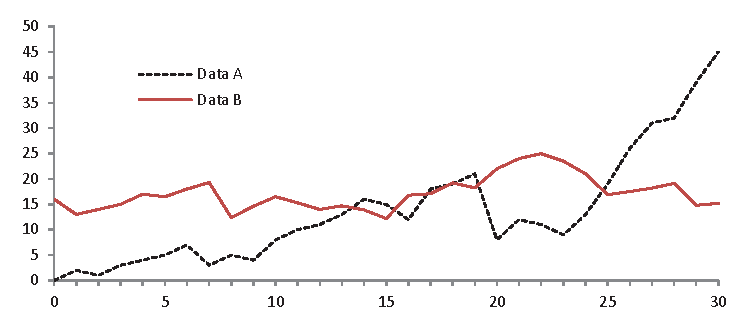
\includegraphics[width=\textwidth]{fig1.eps}
\caption{A figure caption is always placed below the illustration.
Please note that short captions are centered, while long ones are
justified by the macro package automatically.} \label{fig1}
\end{figure}

\begin{theorem}
This is a sample theorem. The run-in heading is set in bold, while
the following text appears in italics. Definitions, lemmas,
propositions, and corollaries are styled the same way.
\end{theorem}
%
% the environments 'definition', 'lemma', 'proposition', 'corollary',
% 'remark', and 'example' are defined in the LLNCS documentclass as well.
%
\begin{proof}
Proofs, examples, and remarks have the initial word in italics,
while the following text appears in normal font.
\end{proof}
For citations of references, we prefer the use of square brackets
and consecutive numbers. Citations using labels or the author/year
convention are also acceptable. The following bibliography provides
a sample reference list with entries for journal
articles~\cite{ref_article1}, an LNCS chapter~\cite{ref_lncs1}, a
book~\cite{ref_book1}, proceedings without editors~\cite{ref_proc1},
and a homepage~\cite{ref_url1}. Multiple citations are grouped
\cite{ref_article1,ref_lncs1,ref_book1},
\cite{ref_article1,ref_book1,ref_proc1,ref_url1}.
%
% ---- Bibliography ----
%
% BibTeX users should specify bibliography style 'splncs04'.
% References will then be sorted and formatted in the correct style.
%
% \bibliographystyle{splncs04}
% \bibliography{mybibliography}
%
\bibliographystyle{splncs04}
\bibliography{samplepaper.bib}
%\begin{thebibliography}{8}
%\bibitem{ref_article1}
%Author, F.: Article title. Journal \textbf{2}(5), 99--110 (2016)
%
%\bibitem{ref_lncs1}
%Author, F., Author, S.: Title of a proceedings paper. In: Editor,
%F., Editor, S. (eds.) CONFERENCE 2016, LNCS, vol. 9999, pp. 1--13.
%Springer, Heidelberg (2016). \doi{10.10007/1234567890}
%
%\bibitem{ref_book1}
%Author, F., Author, S., Author, T.: Book title. 2nd edn. Publisher,
%Location (1999)
%
%\bibitem{ref_proc1}
%Author, A.-B.: Contribution title. In: 9th International Proceedings
%on Proceedings, pp. 1--2. Publisher, Location (2010)
%
%\bibitem{test1}
%@inproceedings{kamishima2012fairness,
%  title={Fairness-aware classifier with prejudice remover regularizer},
%  author={Kamishima, Toshihiro and Akaho, Shotaro and Asoh, Hideki and Sakuma, Jun},
%  booktitle={Joint European Conference on Machine Learning and Knowledge Discovery in Databases},
%  pages={35--50},
%  year={2012},
%  organization={Springer}
%}
%
%
%\bibitem{ref_url1}
%LNCS Homepage, \url{http://www.springer.com/lncs}. Last accessed 4
%Oct 2017
%\end{thebibliography}
\end{document}
